\begin{figure}[ht!]
\centering
\resizebox{0.221\textwidth}{!}{
    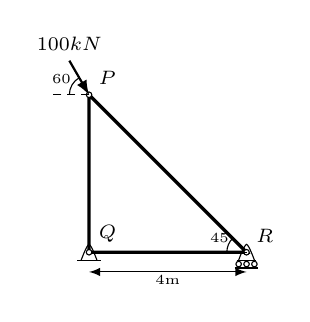
\begin{tikzpicture}
    \draw[black, very thick] (0,0) to (2,0) to (0,2) to (0,0);
    \filldraw[fill=white, draw=black] (0,0) circle (1pt) node[anchor=south west]{\scriptsize $Q$};
    \filldraw[fill=white, draw=black] (2,0) circle (1pt) node[anchor=south west]{\scriptsize $R$};
    \filldraw[fill=white, draw=black] (0,2) circle (1pt) node[anchor=south west]{\scriptsize $P$};
    \draw[black, thick, latex-] (0,2) to ++(-0.25,{sqrt(3)/4}) node[anchor=south]{\scriptsize$100kN$};
    \draw[black, densely dashed] (0,2) to ++(-0.5,0);
    \draw[thin] (-0.25, 2) arc[start angle=180, end angle=120, radius=0.25cm];
    \draw[thin] (1.75, 0) arc[start angle=180, end angle=135, radius=0.25cm];
    \draw[thin] plot [smooth] coordinates {(1.9, -0.1) (2, 0.1) (2.1, -0.1) };
    \draw[thin] (1.875,-0.1) to ++(+0.25,0);
    \draw[thin] (1.9, -0.15) circle (1pt);
    \draw[thin] (2.1, -0.15) circle (1pt);
    \draw[thin] (2.0, -0.15) circle (1pt);
    \draw[thin] (1.85,-0.2) to ++(+0.3,0);
    \draw[thin] plot [smooth] coordinates {(-0.1, -0.1) (0, 0.1) (0.1, -0.1)};
    \draw[thin] (-0.15,-0.1) to ++(+0.3,0);
    \draw[black] (2,0) to ++(-0.1,0) node[anchor=south east]{\tiny 45};
    \node at (-0.35, 2.2) {\tiny 60};
    \draw[black, latex-latex] (0,-0.25) to (2,-0.25);
    \node at (1,-0.35) {\tiny 4m};
\end{tikzpicture}
}
\end{figure}